\documentclass[aspectratio=169]{beamer}
\usepackage{colortbl,tabularx,mathrsfs,calligra}
\usepackage{amsmath,amsfonts,amssymb,amsthm}
\usepackage{ragged2e}
\usepackage[bahasa]{babel}
\usepackage{tikz}
\usepackage{caption}
\usepackage{wrapfig}
\usepackage{multirow}
\usepackage{multicol}
\usepackage{array}
\usepackage{ulem}
\usepackage{pgfplots, tkz-euclide,calc}
\pgfplotsset{compat=1.18}
\usepackage{listings}

\graphicspath{{C:/Users/teoso/OneDrive/Documents/Tugas Kuliah/Template Math Depart/}{./foto/}}

\definecolor{HIMAmuda}{HTML}{01D1FD}
\definecolor{HIMAtua}{HTML}{02016A}
\definecolor{HIMAabu}{HTML}{CBCBCC}
\definecolor{PastelGreen}{HTML}{77DD77}

\usetheme{Madrid}

\setbeamercolor{palette primary}{bg=HIMAtua,fg=white}
\setbeamercolor{palette secondary}{bg=HIMAmuda,fg=black}
\setbeamercolor{palette tertiary}{bg=HIMAabu,fg=black}
\setbeamercolor{palette quaternary}{bg=HIMAmuda,fg=white}
\setbeamercolor{structure}{fg=HIMAmuda} % itemize, enumerate, etc
\setbeamercolor{section in toc}{fg=HIMAtua} % TOC sections
\setbeamercolor{bibliography item}{parent=palette secondary}
\setbeamercolor*{bibliography entry author}{parent=section in toc}

\usetikzlibrary{shapes.geometric, arrows}

\tikzstyle{startstop} = [ellipse, minimum width=1cm, minimum height=1cm,text centered, draw=black, fill=red!30]
\tikzstyle{process} = [rectangle, minimum width=2cm, minimum height=1cm, text centered, draw=black, fill=blue!30]
\tikzstyle{decision} = [diamond, minimum width=1cm, minimum height=1cm, text centered, draw=black, fill=blue!50]
\tikzstyle{arrow} = [thick,->,>=stealth]

\newcolumntype{L}[1]{>{\raggedright\let\newline\\\arraybackslash\hspace{0pt}}m{#1}}
\newcolumntype{C}[1]{>{\centering\let\newline\\\arraybackslash\hspace{0pt}}m{#1}}
\newcolumntype{R}[1]{>{\raggedleft\let\newline\\\arraybackslash\hspace{0pt}}m{#1}}

\usefonttheme{professionalfonts}
\setbeamertemplate{theorems}[numbered]
\setbeamertemplate{bibliography item}{\insertbiblabel}
% \setbeamercovered{transparent}


\theoremstyle{definition}
% \numberwithin{subsection}{section}
\newtheorem{definisi}{Definisi}
\newtheorem{teorema}{Teorema}
\newtheorem{contoh}{Contoh}
\newtheorem{latihan}{Latihan}
\newcommand{\R}{\mathbb{R}}
\newcommand{\N}{\mathbb{N}}
\newcommand{\Z}{\mathbb{Z}}
\newcommand{\C}{\mathbb{C}}


\AtBeginEnvironment{contoh}{%
\setbeamercolor{block title}{use=example text,fg=white,bg=example text.fg!75!black}
\setbeamercolor{block body}{parent=normal text,use=block title example,bg=block title example.bg!10!bg}
\setbeamercolor{item}{fg=example text.fg}
}
\AtBeginEnvironment{definisi}{
\setbeamercolor{block title}{fg=white,bg=HIMAtua}
\setbeamercolor{block body}{parent=normal text,bg=HIMAtua!30!white}
\setbeamercolor{item}{fg=HIMAtua}
}
\AtBeginEnvironment{latihan}{%
  \setbeamercolor{block title}{fg=white,bg=yellow!50!orange} 
  \setbeamercolor{block body}{parent=normal text,bg=yellow!30!white} 
  \setbeamercolor{item}{fg=yellow!50!orange}
}
\AtBeginEnvironment{teorema}{
  \setbeamercolor{block title}{bg=darkgray,fg=white}
  \setbeamercolor{block body}{parent=pallette tertiary,bg=HIMAabu!30!white}
  \setbeamercolor{item}{fg=white}
}

\date{Sabtu, 26 April 2025}
\title[Teori Graf]{Graf dan Pohon}
\author[Tew \& Haf]{Teosofi Hidayah Agung\\Hafidz Mulia}

\begin{document}
\begin{frame}
    \titlepage
\end{frame}

\begin{frame}{Daftar Isi}
  \tableofcontents
\end{frame}

\section{Graf}
\begin{frame}
  \frametitle{\insertsection}
  \begin{definisi}
    \textbf{Graf} adalah himpunan pasangan terurut dari dua himpunan, yaitu himpunan titik dan himpunan sisi. Graf dinyatakan dengan $G = (V, E)$, di mana $V$ adalah himpunan titik dan $E$ adalah himpunan sisi yang menghubungkan antara 2 titik (tidak harus berbeda). 
  \end{definisi}
  \begin{center}
    
  
  \begin{multicols}{4}
    \begin{tikzpicture}[scale=1, every node/.style={circle, draw, fill=black, minimum size=5pt,inner sep=0pt}]
      % Nodes
      \node (A) at (0,1) {};
      \node (B) at (-1,0) {};
      \node (C) at (0,0) {};
      \node (D) at (1,0) {};
      \node (E) at (0,-1) {};
      \node (F) at (1,-1) {};
      
      % Edges
      \draw (A) -- (B);
      \draw (A) -- (C);
      \draw (A) -- (D);
      \draw (B) -- (E);
      \draw (C) -- (E);
      \draw (D) -- (E);
      \draw (C) -- (F);
      \draw (D) -- (F);
  \end{tikzpicture}\\
  \begin{tikzpicture}[scale=1, every node/.style={circle, draw, fill=black, minimum size=5pt,inner sep=0pt}]
    
      % Nodes
      \node (A) at (0,1) {};
      \node (B) at (-1,0) {};
      \node (C) at (0,0) {};
      \node (D) at (1,0) {};
      \node (E) at (0,-1) {};
      
      %Edges
      \draw (A) -- (C);
      \draw (B) -- (C);
      \draw (C) -- (D);
      \draw (C) -- (E);

  \end{tikzpicture}\\  
  \begin{tikzpicture}[scale=1,->, >=stealth, auto, every node/.style={circle, draw, fill=black, minimum size=5pt,inner sep=0pt}]
    % Nodes
    \node (A) at (0,1) {};
    \node (B) at (0,0) {};
    \node (C) at (1,-1) {};
    \node (D) at (-1,-1) {};
    
    % Edges
    \draw (A) -- (B);
    \draw (A) -- (C);
    \draw (A) -- (D);
    \draw (C) to[bend left]  (D);
    \draw (D) to[bend left]  (C);
    \draw (B) to[loop below] (B);
  \end{tikzpicture}\\  
  \begin{tikzpicture}[scale=1, every node/.style={circle, draw, fill=black, minimum size=5pt,inner sep=0pt}]
    % Nodes
    \node (A) at (0,0) {};
    \node (B) at (1,0) {};
    \node (C) at (2,0) {};
    \node (D) at (2,-1) {};
    \node (E) at (1,-1) {};
    \node (F) at (0,-1) {};
    \node (G) at (1,-2) {};
    
    % Edges
    \draw (A) -- node[draw=none,fill=none,midway, above,sloped,gray] {\tiny 1} (B);
    \draw (B) -- node[draw=none,fill=none,midway, above,sloped,gray] {\tiny 2}(C);
    \draw (C) -- node[draw=none,fill=none,midway, above,sloped,gray] {\tiny 5}(D);
    \draw (C) -- node[draw=none,fill=none,midway, above,sloped,gray] {\tiny 13}(E);
    \draw (E) -- node[draw=none,fill=none,midway, above,sloped,gray] {\tiny 4}(F);
    \draw (E) -- node[draw=none,fill=none,midway, above,sloped,gray] {\tiny 9}(B);
    \draw (E) -- node[draw=none,fill=none,midway, above,sloped,gray] {\tiny 10}(G);
    \draw (F) -- node[draw=none,fill=none,midway, above,sloped,gray] {\tiny 2}(G);

  \end{tikzpicture}
  \end{multicols}
  \begin{figure}
    \centering
    \caption{Contoh-contoh graf}
  \end{figure}
\end{center}
\end{frame}

\subsection{Terminologi}
\begin{frame}
  \frametitle{\insertsection}
  \framesubtitle{\insertsubsection}
  \begin{enumerate}
    \item \textbf{Simpul (Vertex)} adalah titik pada graf yang dihubungkan oleh sisi.
    \item \textbf{Sisi (Edge)} adalah garis yang menghubungkan dua simpul pada graf.
    \item \textbf{Derajat (Degree)} adalah banyaknya sisi yang terhubung pada suatu simpul. Derajat dari simpul $v$ dinyatakan dengan $d(v)$.
    \item \textbf{Bertetangga (Adjacent)}, dua simpul $u$ dan $v$ dikatakan bertetangga jika terdapat sisi yang menghubungkan keduanya.
    \item \textbf{Bersisian (Incident)}, sisi $e$ dikatakan bersisian dengan simpul $v$ jika $u$ adalah salah satu ujung dari sisi $e$.
    \item \textbf{Lintasan (Path)} adalah urutan simpul yang dihubungkan oleh sisi.
    \item \textbf{Sirkuit (Circuit)} adalah lintasan yang dimulai dan diakhiri pada simpul yang sama.
    \item \textbf{Siklus (Cycle)} sama seperti sirkuit, namun dengan syarat tidak boleh mengunjungi simpul yang sama lebih dari sekali (dalam konteks graf berarah).
  \end{enumerate}
\end{frame}

\begin{frame}
  \frametitle{\insertsection}
  \framesubtitle{\insertsubsection}
  Graf banyak macamnya dan dibedakan menjadi beberapa jenis, antara lain:
  \begin{block}{Tipe-tipe Graf}
    \begin{itemize}
      \item \textbf{Graf sederhana} adalah graf yang tidak memiliki sisi ganda dan tidak memiliki loop.
      \item \textbf{Graf berarah} adalah graf yang memiliki sisi yang menghubungkan dua titik dengan arah tertentu.
      \item \textbf{Graf berbobot} adalah graf yang memiliki bobot pada setiap sisi.
      \item \textbf{Graf terhubung} adalah graf yang memiliki jalur antara setiap pasangan titik.
    \end{itemize}
  \end{block}
\end{frame}

\begin{frame}
  \frametitle{\insertsection}
  \framesubtitle{\insertsubsection}
  Contoh nama-nama graf yang umum:
  \begin{enumerate}
    \item \textbf{Graf lengkap} adalah graf yang memiliki sisi antara setiap pasangan simpul. Dinotasikan $K_n$, di mana $n$ adalah jumlah simpul.
    \item \textbf{Graf bipartit} adalah graf yang simpul-simpulnya dapat dibagi menjadi dua himpunan sehingga setiap sisi menghubungkan simpul dari himpunan yang berbeda.
    \item \textbf{Graf planar} adalah graf yang dapat digambar di bidang tanpa sisi yang saling berpotongan. 
    \item \textbf{Graf Hamiltonian} 
    \item \textbf{Graf Euler}
  \end{enumerate}
\end{frame}

\begin{frame}
  \frametitle{\insertsection}
  \begin{teorema}[Lemma Jabat Tangan]
    Misalkan $G=(V,E)$ adalah graf tak berarah hingga. Maka 
    \[\sum_{v \in V} d(v) = 2|E|.\]
    atau bisa dibilang jumlah derajat semua simpul sama dengan dua kali banyak sisi (genap).
  \end{teorema}
\end{frame}

\begin{frame}
  \frametitle{\insertsection}
  Mungkinkah dibuat \textbf{graf sederhana dan terhubung} dengan 5 simpul dengan derajat masing-masing simpul adalah:
  \begin{enumerate}
      \item 2, 3, 1, 1, 2
      \item 2, 3, 3, 4, 4
      \item 5, 2, 3, 2, 4
      \item 4, 4, 3, 2, 3
      \item 3, 3, 2, 3, 2
      \item 4, 4, 1, 3, 2
  \end{enumerate}
\end{frame}

\subsection{Graf Hamiltonian}
\begin{frame}
  \frametitle{\insertsection}
  \framesubtitle{\insertsubsection}
  \begin{definisi}
    \textbf{Lintasan Hamiltonian} adalah lintasan yang mengunjungi setiap simpul tepat satu kali.
  \end{definisi}
  Carilah lintasan Hamiltonian pada graf berikut:
  \begin{center}
    \only<1>{\begin{multicols}{3}
      \begin{tikzpicture}[every node/.style={draw,circle, font=\tiny\bfseries, fill=black, minimum size=5pt,inner sep=0pt}, scale=0.8]
        % Node positions
        \node (A) at (0,2) {};
        \node (B) at (2,2) {};
        \node (C) at (4,2) {};
        \node (D) at (0,0) {};
        \node (E) at (2,0) {};
        \node (F) at (4,0) {};
      
        \draw (A) -- (B);
        \draw (B) -- (C);
        \draw (A) -- (D);
        \draw (D) -- (E);
        \draw (C) -- (F);
        \draw (B) -- (E);
        \draw (B) -- (F);
        \draw (C) -- (E);
        \draw (C) -- (F);
      \end{tikzpicture}\\
      \begin{tikzpicture}[every node/.style={draw,circle, font=\tiny\bfseries, fill=black, minimum size=5pt,inner sep=0pt}, scale=0.5]
        % Node positions
        \node (A) at (2,2) {};
        \node (B) at (-2,2) {};
        \node (C) at (-1,1) {};
        \node (D) at (1,1) {};
        \node (E) at (2,-2) {};
        \node (F) at (-2,-2) {};
        \node (G) at (-1,-1) {};
        \node (H) at (1,-1) {};
      
        \draw (A) -- (B);
        \draw (B) -- (C);
        \draw (A) -- (E);
        \draw (F) -- (G);
        \draw (B) -- (F);
        \draw (G) -- (H);
        \draw (C) -- (D);
        \draw (D) -- (H);
        \draw (C) -- (G);
        \draw (H) -- (E);
        \draw (E) -- (F);
        \draw (A) -- (D);

      \end{tikzpicture}\\
      \begin{tikzpicture}[every node/.style={draw,circle, font=\tiny\bfseries, fill=black, minimum size=5pt,inner sep=0pt}, scale=0.5]
        \node (A) at (0,2) {};
        \node (B) at (2,4) {};
        \node (C) at (4,3) {};
        \node (D) at (5,1) {};
        \node (E) at (2,0) {};
        \node (F) at (2,1.5) {};

        % Edges - black
        \draw[black] (A) -- (B);
        \draw[black] (B) -- (C);
        \draw[black] (C) -- (D);
        \draw[black] (D) -- (E);
        \draw[black] (E) -- (A);
        \draw[black] (A) -- (F);
        \draw[black] (B) -- (F);
        \draw[black] (C) -- (F);
        \draw[black] (F) -- (D);
      \end{tikzpicture}
    \end{multicols}}
    \only<2>{\begin{multicols}{3}
      \begin{tikzpicture}[every node/.style={circle, font=\tiny\bfseries, fill=red, minimum size=5pt,inner sep=0pt}, scale=0.8]
        % Node positions
        \node (A) at (0,2) {};
        \node (B) at (2,2) {};
        \node (C) at (4,2) {};
        \node (D) at (0,0) {};
        \node (E) at (2,0) {};
        \node (F) at (4,0) {};
      
        \draw (A) -- (B);
        \draw (B) -- (C);
        \draw (A) -- (D);
        \draw (D) -- (E);
        \draw (C) -- (F);
        \draw (B) -- (E);
        \draw (B) -- (F);
        \draw (C) -- (E);
        \draw (C) -- (F);

        \draw[thick,red] (A) -- (B) -- (F) -- (C) -- (E) -- (D);
      \end{tikzpicture}\\
      \begin{tikzpicture}[every node/.style={circle, font=\tiny\bfseries, fill=red, minimum size=5pt,inner sep=0pt}, scale=0.5]
        % Node positions
        \node (A) at (2,2) {};
        \node (B) at (-2,2) {};
        \node (C) at (-1,1) {};
        \node (D) at (1,1) {};
        \node (E) at (2,-2) {};
        \node (F) at (-2,-2) {};
        \node (G) at (-1,-1) {};
        \node (H) at (1,-1) {};
      
        \draw (A) -- (B);
        \draw (B) -- (C);
        \draw (A) -- (E);
        \draw (F) -- (G);
        \draw (B) -- (F);
        \draw (G) -- (H);
        \draw (C) -- (D);
        \draw (D) -- (H);
        \draw (C) -- (G);
        \draw (H) -- (E);
        \draw (E) -- (F);
        \draw (A) -- (D);

        \draw[thick,red] (A) -- (B) -- (C) -- (G) -- (F) -- (E) -- (H) -- (D);
      \end{tikzpicture}\\
      \begin{tikzpicture}[every node/.style={circle, font=\tiny\bfseries, fill=red, minimum size=5pt,inner sep=0pt}, scale=0.5]
        \node (A) at (0,2) {};
        \node (B) at (2,4) {};
        \node (C) at (4,3) {};
        \node (D) at (5,1) {};
        \node (E) at (2,0) {};
        \node (F) at (2,1.5) {};

        % Edges - black
        \draw[black] (A) -- (B);
        \draw[black] (B) -- (C);
        \draw[black] (C) -- (D);
        \draw[black] (D) -- (E);
        \draw[black] (E) -- (A);
        \draw[black] (A) -- (F);
        \draw[black] (B) -- (F);
        \draw[black] (C) -- (F);
        \draw[black] (F) -- (D);

        \draw[thick,red] (A) -- (B) -- (F) -- (C) -- (D) -- (E);
      \end{tikzpicture}
    \end{multicols}}
  \end{center}
\end{frame}

\begin{frame}
  \frametitle{\insertsection}
  \framesubtitle{\insertsubsection}
  \begin{definisi}
    \textbf{Sirkuit Hamiltonian} adalah sirkuit yang mengunjungi setiap simpul tepat satu kali (kecuali titik awal dan akhir). 
  \end{definisi}
  Carilah sirkuit Hamiltonian pada graf berikut:
  \begin{center}
    \only<1>{\begin{multicols}{3}
      \begin{tikzpicture}[every node/.style={draw,circle, font=\tiny\bfseries, fill=black, minimum size=5pt,inner sep=0pt}, scale=0.8]
        % Node positions
        \node (A) at (0,2) {};
        \node (B) at (2,2) {};
        \node (C) at (4,2) {};
        \node (D) at (0,0) {};
        \node (E) at (2,0) {};
        \node (F) at (4,0) {};
      
        \draw (A) -- (B);
        \draw (B) -- (C);
        \draw (A) -- (D);
        \draw (D) -- (E);
        \draw (C) -- (F);
        \draw (B) -- (E);
        \draw (B) -- (F);
        \draw (C) -- (E);
        \draw (C) -- (F);
      \end{tikzpicture}\\
      \begin{tikzpicture}[every node/.style={draw,circle, font=\tiny\bfseries, fill=black, minimum size=5pt,inner sep=0pt}, scale=0.5]
        % Node positions
        \node (A) at (2,2) {};
        \node (B) at (-2,2) {};
        \node (C) at (-1,1) {};
        \node (D) at (1,1) {};
        \node (E) at (2,-2) {};
        \node (F) at (-2,-2) {};
        \node (G) at (-1,-1) {};
        \node (H) at (1,-1) {};
      
        \draw (A) -- (B);
        \draw (B) -- (C);
        \draw (A) -- (E);
        \draw (F) -- (G);
        \draw (B) -- (F);
        \draw (G) -- (H);
        \draw (C) -- (D);
        \draw (D) -- (H);
        \draw (C) -- (G);
        \draw (H) -- (E);
        \draw (E) -- (F);
        \draw (A) -- (D);

      \end{tikzpicture}\\
      \begin{tikzpicture}[every node/.style={draw,circle, font=\tiny\bfseries, fill=black, minimum size=5pt,inner sep=0pt}, scale=0.5]
        \node (A) at (0,2) {};
        \node (B) at (2,4) {};
        \node (C) at (4,3) {};
        \node (D) at (5,1) {};
        \node (E) at (2,0) {};
        \node (F) at (2,1.5) {};

        % Edges - black
        \draw[black] (A) -- (B);
        \draw[black] (B) -- (C);
        \draw[black] (C) -- (D);
        \draw[black] (D) -- (E);
        \draw[black] (E) -- (A);
        \draw[black] (A) -- (F);
        \draw[black] (B) -- (F);
        \draw[black] (C) -- (F);
        \draw[black] (F) -- (D);
      \end{tikzpicture}
    \end{multicols}}
    \only<2>{\begin{multicols}{3}
      \begin{tikzpicture}[every node/.style={circle, font=\tiny\bfseries, fill=red, minimum size=5pt,inner sep=0pt}, scale=0.8]
        % Node positions
        \node (A) at (0,2) {};
        \node (B) at (2,2) {};
        \node (C) at (4,2) {};
        \node (D) at (0,0) {};
        \node (E) at (2,0) {};
        \node (F) at (4,0) {};
      
        \draw (A) -- (B);
        \draw (B) -- (C);
        \draw (A) -- (D);
        \draw (D) -- (E);
        \draw (C) -- (F);
        \draw (B) -- (E);
        \draw (B) -- (F);
        \draw (C) -- (E);
        \draw (C) -- (F);

        \draw[thick,red] (A) -- (B) -- (F) -- (C) -- (E) -- (D) -- cycle;
      \end{tikzpicture}\\
      \begin{tikzpicture}[every node/.style={circle, font=\tiny\bfseries, fill=red, minimum size=5pt,inner sep=0pt}, scale=0.5]
        % Node positions
        \node (A) at (2,2) {};
        \node (B) at (-2,2) {};
        \node (C) at (-1,1) {};
        \node (D) at (1,1) {};
        \node (E) at (2,-2) {};
        \node (F) at (-2,-2) {};
        \node (G) at (-1,-1) {};
        \node (H) at (1,-1) {};
      
        \draw (A) -- (B);
        \draw (B) -- (C);
        \draw (A) -- (E);
        \draw (F) -- (G);
        \draw (B) -- (F);
        \draw (G) -- (H);
        \draw (C) -- (D);
        \draw (D) -- (H);
        \draw (C) -- (G);
        \draw (H) -- (E);
        \draw (E) -- (F);
        \draw (A) -- (D);

        \draw[thick,red] (A) -- (B) -- (C) -- (G) -- (F) -- (E) -- (H) -- (D) -- cycle;
      \end{tikzpicture}\\
      \begin{tikzpicture}[every node/.style={circle, font=\tiny\bfseries, fill=red, minimum size=5pt,inner sep=0pt}, scale=0.5]
        \node (A) at (0,2) {};
        \node (B) at (2,4) {};
        \node (C) at (4,3) {};
        \node (D) at (5,1) {};
        \node (E) at (2,0) {};
        \node (F) at (2,1.5) {};

        % Edges - black
        \draw[black] (A) -- (B);
        \draw[black] (B) -- (C);
        \draw[black] (C) -- (D);
        \draw[black] (D) -- (E);
        \draw[black] (E) -- (A);
        \draw[black] (A) -- (F);
        \draw[black] (B) -- (F);
        \draw[black] (C) -- (F);
        \draw[black] (F) -- (D);

        \draw[thick,red] (A) -- (B) -- (F) -- (C) -- (D) -- (E) -- cycle;
      \end{tikzpicture}
    \end{multicols}}
  \end{center}
\end{frame}

\begin{frame}
  \frametitle{\insertsection}
  \framesubtitle{\insertsubsection}
  Secara umum dapat disimpulkan bahwa graf Hamiltonian haruslah terhubung. 
  \begin{teorema}[Dirac's]
    Untuk graf terhubung $G$ dengan $n$ simpul dan jika graf tersebut sederhana dan setiap simpul memiliki derajat lebih besar dari atau sama dengan $\frac{n}{2}$, maka $G$ memiliki lintasan dan sirkuit Hamiltonian.
  \end{teorema}
\end{frame}

\subsection{Graf Euler}
\begin{frame}
  \frametitle{\insertsection}
  \framesubtitle{\insertsubsection}
  Ada sebuah kota bernama Königsberg di Prusia (sekarang Kaliningrad di Rusia). Kota ini dipisahkan oleh sungai dan memiliki 4 daratan yang dihubungkan oleh 7 jembatan.

  Pertanyaannya adalah:

  \textbf{Apakah mungkin berjalan mengelilingi kota dengan melewati setiap jembatan tepat satu kali tanpa mengulang, dan kembali ke titik awal?}
  \begin{center}
    \begin{multicols}{3}
      \begin{figure}
        \centering
        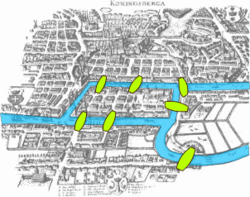
\includegraphics[width=0.3\textwidth]{Seven Bridges of Konigsberg.png}
      \end{figure}
      \begin{figure}
        \centering
        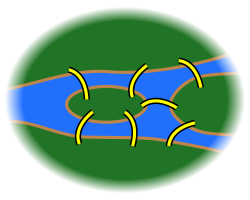
\includegraphics[width=0.3\textwidth]{Ilustrasi Jembatan.png}
      \end{figure}
      \begin{figure}
        \centering
        \begin{tikzpicture}[scale=2, every node/.style={circle, draw, fill=green!50, inner sep=3pt}]
          % Node positions
          \node (A) at (-1,0.8) {};
          \node (B) at (-1,-0.8) {};
          \node (C) at (-1,0) {};
          \node (D) at (0,0) {};

          % Edges
          \draw (A) to[bend left] (C);
          \draw (C) to[bend left] (A);
          \draw (C) to[bend left] (B);
          \draw (B) to[bend left] (C);
          \draw (A) -- (D);
          \draw (B) -- (D);

        \end{tikzpicture}
      \end{figure}
    \end{multicols}
  \end{center}
\end{frame}

\begin{frame}
  \frametitle{\insertsection}
  \framesubtitle{\insertsubsection}
  \begin{definisi}
    \textbf{Lintasan Eulerian} adalah lintasan yang mengunjungi setiap sisi tepat satu kali. 
  \end{definisi}
\end{frame}

\begin{frame}
  \frametitle{\insertsection}
  \framesubtitle{\insertsubsection}
  \begin{definisi}
    \textbf{Sirkuit Eulerian} adalah sirkuit yang mengunjungi setiap sisi tepat satu kali (kecuali titik awal dan akhir). 
  \end{definisi}
  \begin{center}
    
  \end{center}
\end{frame}

\begin{frame}
  \frametitle{\insertsection}
  \framesubtitle{\insertsubsection}
  \begin{teorema}[Euler]
    Suatu graf terhubung $G$ memiliki lintasan Eulerian jika dan hanya jika paling banyak dua simpul memiliki derajat ganjil.
  \end{teorema}
  \begin{teorema}[Euler]
    Suatu graf terhubung $G$ memiliki Sirkuit Eulerian jika dan hanya jika semua simpul memiliki derajat genap.
  \end{teorema}
\end{frame}

\section{Pohon}
\begin{frame}
  \frametitle{\insertsection}
  \begin{definisi}
    \textbf{Pohon (Tree)} adalah graf terhubung yang tidak memiliki siklus.
  \end{definisi}
  \begin{teorema}
    Jika $G$ adalah pohon dengan $n$ simpul, maka $G$ memiliki $n-1$ sisi.
  \end{teorema}
\end{frame}
\end{document}